\documentclass{article}

% if you need to pass options to natbib, use, e.g.:
%     \PassOptionsToPackage{numbers, compress}{natbib}
% before loading neurips_2020

% ready for submission
% \usepackage{neurips_2020}

% to compile a preprint version, e.g., for submission to arXiv, add add the
% [preprint] option:
\usepackage[preprint]{neurips_2020}

% to compile a camera-ready version, add the [final] option, e.g.:
%     \usepackage[final]{neurips_2020}

% to avoid loading the natbib package, add option nonatbib:
%     \usepackage[nonatbib]{neurips_2020}

\usepackage[utf8]{inputenc} % allow utf-8 input
\usepackage[T1]{fontenc}    % use 8-bit T1 fonts
\usepackage{graphicx}
\usepackage{hyperref}       % hyperlinks
\usepackage{url}            % simple URL typesetting
\usepackage{booktabs}       % professional-quality tables
\usepackage{amsmath}
\usepackage{amssymb}
\usepackage{amsfonts}       % blackboard math symbols
\usepackage{nicefrac}       % compact symbols for 1/2, etc.
\usepackage{microtype}      % microtypography
\usepackage{alltt}
\usepackage{listings}
\usepackage{array}
\usepackage[noline, procnumbered]{algorithm2e}
\usepackage{lmodern}
\usepackage{caption}
\usepackage{subcaption}
\usepackage{xcolor}
\newcommand\mycommfont[1]{\footnotesize\ttfamily\textcolor{gray}{#1}}
\SetCommentSty{mycommfont}


\newcommand{\secref}[1]{Section~\ref{#1}}
\newcommand{\tblref}[1]{Table~\ref{#1}}
\newcommand{\figref}[1]{Figure~\ref{#1}}
\newcommand{\thmref}[1]{Theorem~\ref{#1}}
\newcommand{\algref}[1]{Algorithm~\ref{#1}}
\newcommand{\funref}[1]{Function~\ref{#1}}
\newcommand{\listingref}[1]{Listing~\ref{#1}}

\newcommand{\eg}{{\em e.g.}}
\newcommand{\ith}{$i^{th}$}
\newcommand{\cut}[1]{}
\newcommand{\todo}[1]{{\bf\em TODO:} {{\color{red}{#1}}}}

\newcommand{\spd}{\fontfamily{cmr}\textsc{\small StratPD}}
\newcommand{\cspd}{\fontfamily{cmr}\textsc{\small CatStratPD}}
\newcommand{\xnc}{${\bf X}_{\overline{c}}$}
\newcommand{\xnC}{$x_{\overline{C}}$}

%\setlist[enumerate]{itemsep=-1mm}

\title{Technical Report:\\
A Stratification Approach to Partial Dependence for Codependent Variables}

\author{%
  Terence Parr \\
  University of San Francisco\\
  \texttt{parrt@cs.usfca.edu} \\
  \And
  James D. Wilson \\
  University of San Francisco\\
  \texttt{jdwilson4@usfca.edu} \\
}

\begin{document}

\maketitle

\begin{abstract}
\end{abstract}

\section{Introduction}

\begin{figure}[htbp]
\begin{center}
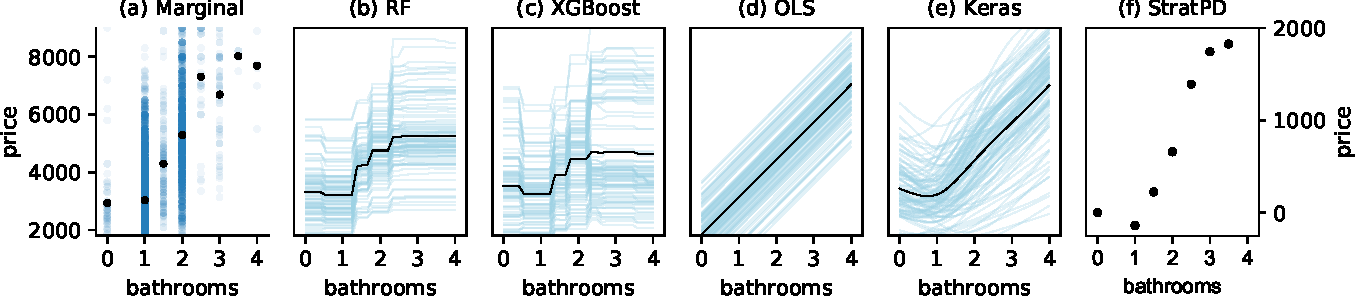
\includegraphics[scale=0.5]{images/bathrooms_vs_price.pdf}
\caption{\footnotesize Plots of bathrooms versus rent price using New York City apartment rent data. (a) marginal plot, (b) PD/ICE plot derived from random forest, (c) PD/ICE plot derived from gradient boosted machine, and (d) PD/ICE plot derived from ordinary least squares regression; sample size is 10,000 observations of \textasciitilde50k. The PD/ICE plots are  different for the same data set, depending on the chosen user model. X['bathrooms'].unique() shows (array([0. , 1. , 1.5, 2. , 2.5, 3. , 3.5, 4. ]),
 array([  54, 8151,  140, 1539,   39,   67,    3,    7])). \spd{} has missing last value, not enough data.}
\label{fig:baths_price}
\end{center}
\end{figure}

partial dependence is important because...

Existing techniques, such as FPD, ICE, ALE, SHAP peer through the lens of a model's predictions. For the same data applying the same technique but using different models, we get different answers, which calls into question the validity of the curves.

key is "all else being equal", which implies you don't want curves affected by other variables. Interaction plots are also very useful, such as ICE, but here our goal is the pure partial dependence curve. In the future, we hope to consider extracting interaction between variables like SHAP.

Many analysts do not need a predictive model nor would they know how to choose, tune, and assess a model. Could also be the case that a technique is not available in the desired deployment environment.  The techniques differ in algorithm simplicity, performance, and ability to isolate codependent variables. a nonparametric technique could also inform which machine learning model to use if a model is desired.

we introduce an ideal definition of partial dependence that does not rely on predictions from a fitted model based upon partial derivatives and then estimate partial derivatives nonparametrically to get partial dependence. The technique seems to isolate variables well and has linear behavior for numeric variables and mildly quadratic behavior for categorical variables in practice. The theoretical complexity is $O(n^2)$ like FPD.

SHAP is mean centered FPD for independent variables, proof in supplemental material.

state up front it only gets pure partial dependence, no interaction and has quadratic theoretical complexity, but it has the advantage that it doesn't require a fitted model.  Sometimes there is an advantage to a model, smoothing etc. But, in many cases lack of model increases the accessibility of the tool to analysts and could prevent nonexpert machine learning practitioners from interpretation errors from poorly fit or tuned models.

\section{Partial dependence without model predictions}

\noindent {\bf Definition 1} The {\em ideal partial dependence} of $y$ on feature $x_j$ for smooth generator function $f:\mathbb{R}^{p} \rightarrow \mathbb{R}$ evaluated at $x_j = z$ is the cumulative sum up to $z$:

\begin{equation}\label{eq:pd}
\text{\it PD}_j(z) = \int_{min(x_j)}^z \frac{\partial y}{\partial x_j} dx_j
\end{equation}

$\text{\it PD}_j(z)$ is the value contributed to $y$ by $x_j$ at $x_j = z$ and $\text{\it PD}_j(min(x_j))=0$. The advantages of this partial dependence definition are that it does not depend on predictions from a fitted model and is insensitive to collinear or otherwise codependent features, unlike the Friedman's original definition that he points out is less accurate for codependent data sets. We will denote Friedman's as $\text{\it FPD}_j$ to distinguish it from this ideal, $\text{\it PD}_j$.

For example, consider quadratic equation $y = x_1^2 + x_2 + 100$ as a generator of data in $[0,3]$. The partial derivatives are $\frac{\partial y}{\partial x_1} = 2 x_1$ and $\frac{\partial y}{\partial x_2} = 1$, giving $\text{\it PD}_1 = x_1^2$ and $\text{\it PD}_2 = x_2$. 

The obvious disadvantage of this feature impact definition is that function $f$, from which $\text{\it PD}_j$ is derived, is unknown in practice, so symbolically computing the partial derivatives is not possible. But, if we could compute accurate partial dependence curves by some other method, then this definition would still represent a viable means to obtain feature impacts. 

\spd{} stratifies a data set into groups of observations that are similar, except in the variable of interest, $x_j$, through the use of a single decision tree. Any fluctuation of the response variable within a group (decision tree leaf) is likely due to $x_j$.  The $\beta_1$ coefficient of a simple local linear regression fit to the $(x_j, y)$ values within a group provides an estimate of $\frac{\partial y}{\partial x_j}$ in that group's $x_j$ range. Averaging the partial derivative estimates across all such groups yields the overall $\frac{\partial y}{\partial x_j}$ partial derivative approximation. The cumulative sum of the estimated partial derivative yields the partial dependence curve. 

\section{Existing work}

FPD

ICE

ALE

SHAP

\section{Experimental results}

\begin{figure}[htbp]
\begin{center}
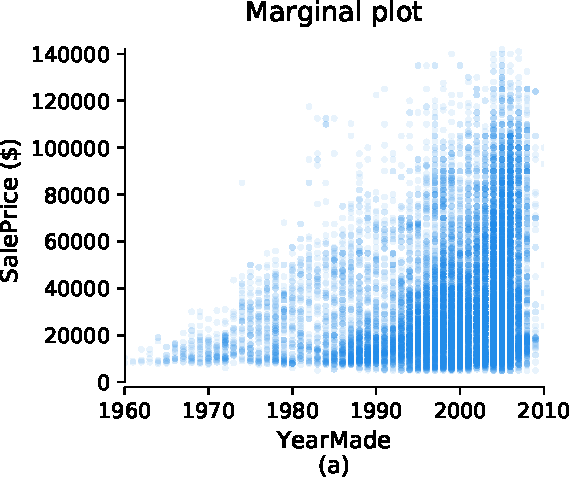
\includegraphics[scale=0.35]{images/bulldozer_YearMade_marginal.pdf}~~
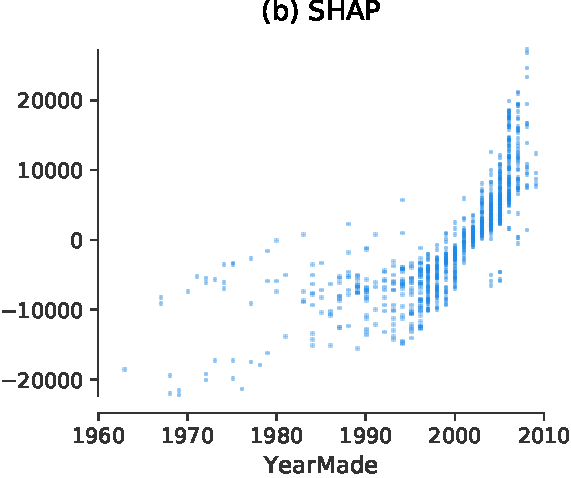
\includegraphics[scale=0.35]{images/bulldozer_YearMade_shap.pdf}~~
\includegraphics[scale=0.35]{images/YearMade_400_ale.pdf}~~
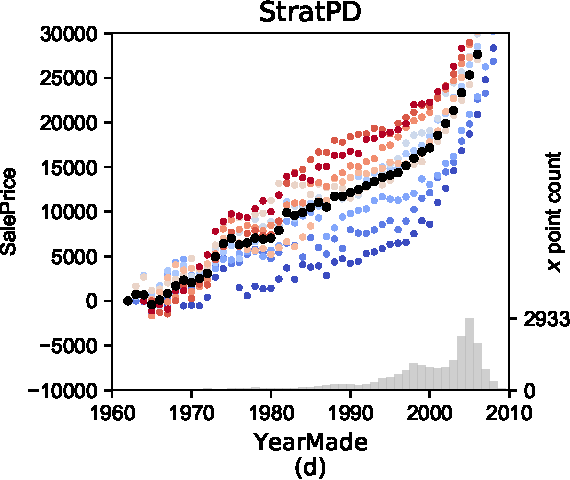
\includegraphics[scale=0.35]{images/bulldozer_YearMade_stratpd.pdf}
\caption{\small (a) Marginal plot of bulldozer {\tt YearMade} versus {\tt SalePrice} using subsample of 20k observations, (b) partial dependence drawn by SHAP interrogating an RF with 40 trees and explaining 1000 values with 100 observations as background data, (c) \spd{} partial dependence.}
\label{fig:shap-stratpd-YearMade}
\end{center}
\end{figure}

\begin{figure}[htbp]
\begin{center}
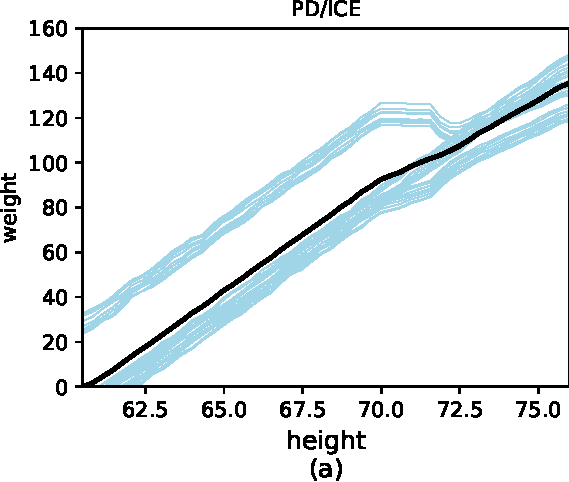
\includegraphics[scale=0.35]{images/height_vs_weight_pdp.pdf}~~
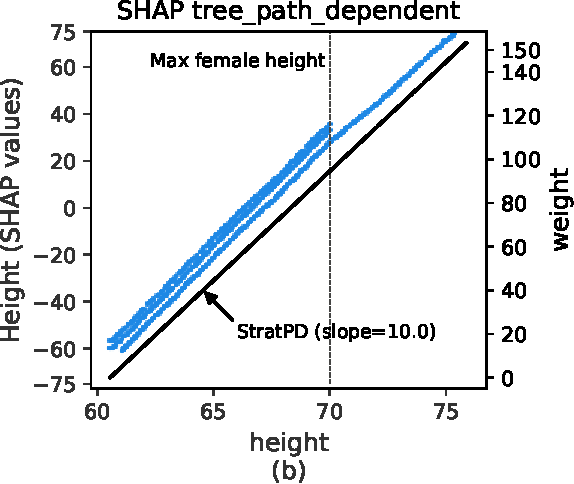
\includegraphics[scale=0.35]{images/weight_tree_path_dependent_shap.pdf}~~
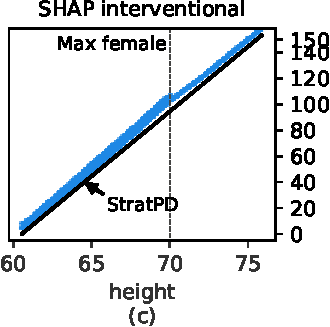
\includegraphics[scale=0.35]{images/weight_interventional_shap.pdf}~~
\includegraphics[scale=0.34]{images/height_300_ale.pdf}~~
\caption{\small SHAP partial dependence plots of response body weight on feature {\tt height} using 2000 synthetic observations from Equation \eqref{eq:weight}. SHAP interrogated an RF with 40 trees and explained all 2000 samples; the interventional case used 100 observations as background data.}
\label{fig:heightweight}
\end{center}
\end{figure}

\begin{figure}[htbp]
\begin{center}
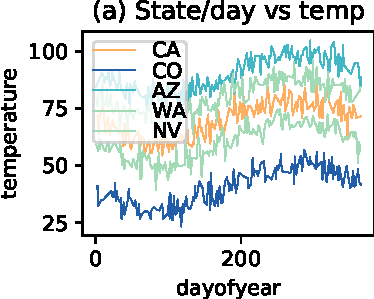
\includegraphics[scale=0.45]{images/dayofyear_vs_temp.pdf}~~
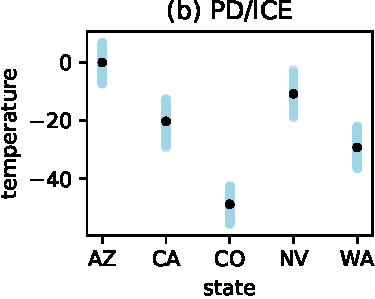
\includegraphics[scale=0.45]{images/state_vs_temp_pdp.pdf}~~
\includegraphics[scale=0.45]{images/state_5_ale.pdf}~~
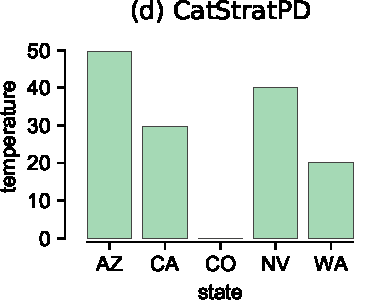
\includegraphics[scale=0.45]{images/state_vs_temp_stratpd.pdf}~~
\caption{\small foo.}
\label{fig:statetemp}
\end{center}
\end{figure}

\begin{figure}[htbp]
\begin{center}
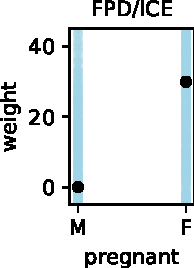
\includegraphics[scale=0.45]{images/pregnant_vs_weight_pdp.pdf}~~
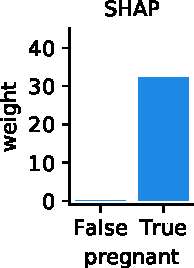
\includegraphics[scale=0.45]{images/pregnant_vs_weight_shap.pdf}~~
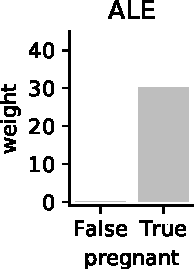
\includegraphics[scale=0.45]{images/pregnant_2_ale.pdf}~~
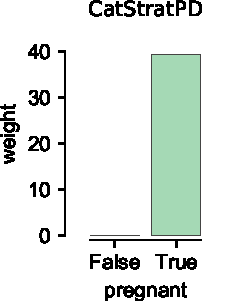
\includegraphics[scale=0.45]{images/pregnant_vs_weight_stratpd.pdf}~~
\caption{\small foo.}
\label{fig:pregnant}
\end{center}
\end{figure}

\begin{figure}[htbp]
\begin{center}
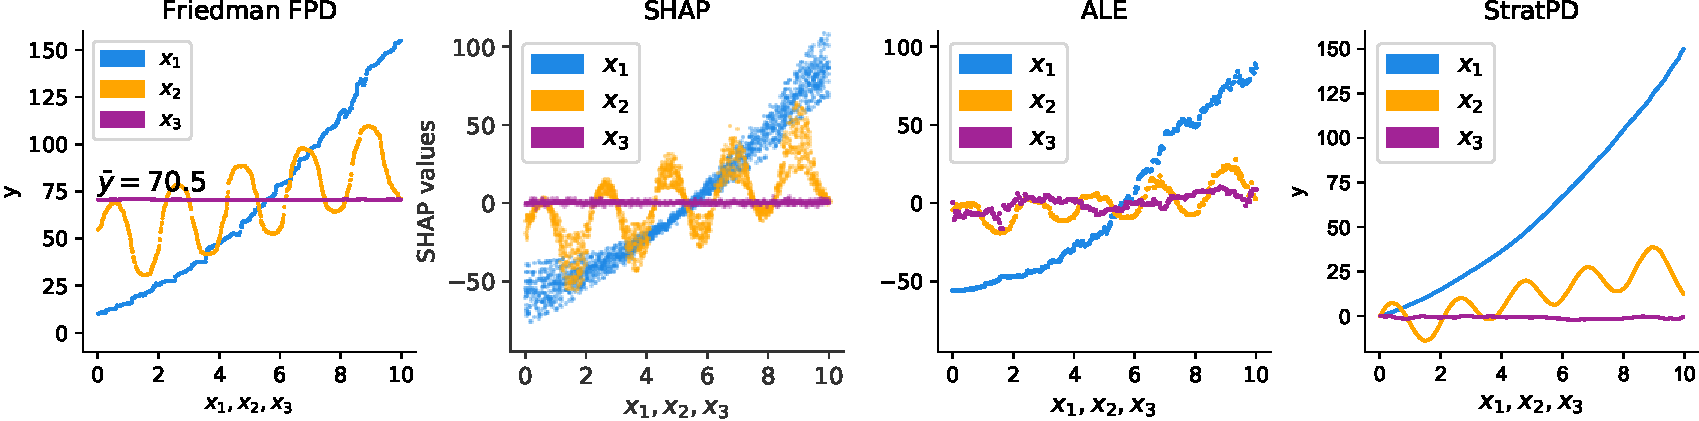
\includegraphics[scale=0.4]{images/interactions.pdf}
\caption{\small $y = x_1^2 + x_1 x_2 + 5 x_1 sin(3 x_2) + 10$ where $x_1,x_2,x_3 \sim U(0,10)$ and $x_3$ does not affect $y$. No noise added.}
\label{fig:interactions}
\end{center}
\end{figure}

\begin{figure}[htbp]
\begin{center}
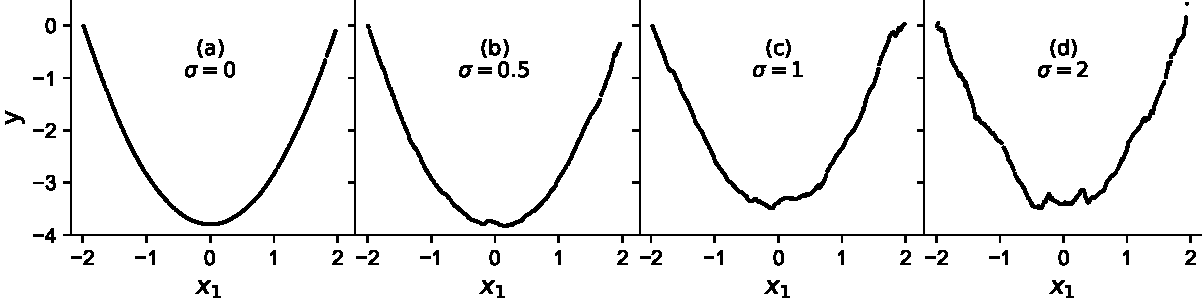
\includegraphics[scale=0.4]{images/noise.pdf}
\caption{\small $y = x_1^2 + x_1 + 10 + N(0,\sigma)$ where $x_1,x_2 \sim U(-2,2)$ and $\sigma \in [0,0.5,1,2]$.}
\label{fig:noise}
\end{center}
\end{figure}


\pagebreak
\section{Algorithms}

{\bf StratPD}\begin{alltt}\small
Fit tree regressor to all but x_c with hyper parameter min_slopes_per_x
For each leaf:
    y bar = Group leaf samples by x_c, computing average y per unique x_c
    dx = discrete difference between adjacent unique x_c
    dy = discrete difference between adjacent average y bar
    add (x[i], x[i+1], dy[i]/dx[i]) for each unique x_c to list D

for each x in unique x_c from X:
    slopes = [slope for (a, b, slope) in D if x >= a and x < b]
    count[x] = |slopes|
    dydx[x] = mean(slopes)

Drop slope estimates computed using fewer than min_slopes_per_x values
pdx = discrete difference between adjacent unique x_c
pdy = cumulative sum of dydx * pdx
return pdx, [0]+pdy  // insert 0 for pdx[0] since sum contributed from beyond left is 0
\end{alltt}

\setlength{\algomargin}{5pt}
\begin{algorithm}[]
\DontPrintSemicolon
\SetAlgorithmName{Algorithm}{List of Algorithms}
\SetAlgoSkip{}
\TitleOfAlgo{{\em StratPD}}
\KwIn{{\bf X}, {\bf y}, c, {\it min\_samples\_leaf}, {\it min\_slopes\_per\_x}}
\KwOut{$\bf pdx, pdy$: Unique $x_c$, partial dependence values across $x_c$}
$T$ := Decision tree regressor fit to (\xnc{}, $\bf y$) with hyper-parameter: ${\it min\_samples\_leaf}$\;
\For{each leaf $l \in T$}{
        $({\bf x}_l, {\bf y}_l)$ = $\{(x_c^{(i)},  y^{(i)})\}_{i \in l}$\tcp*{\it Get leaf samples}
        {\bf ux} := $unique({\bf x}_l)$\\
	$\bar{\bf y}$ := Group leaf records $({\bf x}_l, {\bf y}_l)$ by value of ${\bf x}_l$, computing $\bar{y}$ per unique value\\
	${\bf dx}$ := ${\bf ux}^{(i+1)} - {\bf ux}^{(i)}_{i=1..|{\bf ux}|-1}$\tcp*{\it Discrete difference}
	${\bf dy}$ := $\bar{\bf y}^{(i+1)} - \bar{\bf y}^{(i)}_{i=1..|{\bf ux}|-1}$\\
	Add tuples ${({\bf ux}^{(i)}, {\bf ux}^{(i+1)},~ {\bf dy}^{(i)}/{\bf dx}^{(i)})}_{i=1..|{\bf ux}|-1}$ to list ${\bf d}$\\
}
$\bf ux$ := $unique(\{x_c^{(i)}\}_{i=1..n})$\\
\For{each $x \in {\bf ux}$\tcp*{\it Counts slopes, compute average slope per unique $x_c$ value}}{
	$slopes$ := [$slope$ for $(a,b,slope) \in \bf d$ if $x \ge a$ and $x <b$]\\
	${\bf c}_x$ := $|slopes|$\\
	${\bf dydx}_x$ := $\overline{slopes}$\\
}
${\bf dydx}$ := ${\bf dydx}[{\bf c} \ge min\_slopes\_per\_x]$\tcp*{\it Drop slope estimates computed from too few}
${\bf ux}$ := ${\bf ux}[{\bf c} \ge min\_slopes\_per\_x]$\\
$\bf pdx$ := ${\bf ux}^{(i+1)} - {\bf ux}^{(i)}_{i=1..|{\bf ux}|-1}$\\
$\bf pdy$ := [0] + cumulative\_sum(${\bf dydx} * \bf pdx$)~~~\tcp*{\it integrate, inserting 0 for leftmost $x_c$}
\Return{$\bf pdx, pdy$}
\label{alg:CatStratPD}
\end{algorithm}

\pagebreak

{\bf CatStratPD}\begin{alltt}\small
Fit tree regressor to all but x_c with hyper parameter min_slopes_per_x
For each leaf:
    y bar = Group leaf samples by categories of x_c, computing average y per unique category x_c
    Compute unique categories and counts per category
    refcat is randomly chosen category from x_c
    For each unique category x in leaf:
        delta[cat,leaf] = Subtract y for refcat from all y bar (refcat delta will be 0)
end
Let Avg[cat] be vector with running sum mapping category to count
work = set of leaf indexes
while more work and something changed and less than max iterations:
    for each leaf in leaves:
        if cat in delta[:,leaf] intersects with Avg:
            j = random category in intersection
            adjust delta[:,leaf] to be relative to j so delta[j,leaf]==0 then add Avg[j] so comparable
            merge into Avg
    work -= all j merged this iteration
\end{alltt}

\setlength{\algomargin}{5pt}
\begin{algorithm}[]
\DontPrintSemicolon
\SetAlgorithmName{Algorithm}{List of Algorithms}
\SetAlgoSkip{}
\TitleOfAlgo{{\em CatStratPD}}
\KwIn{${\bf X}, {\bf y}, c, {\it min\_samples\_leaf}$}
\KwOut{$\begin{array}[t]{l}
\Delta^{(k)} = \text{category } k \text{'s effect on } y \text{ where } mean(\Delta^{(k)})=0\\
n^{(k)} = \text{number of supported observations per category $k$}\\
\end{array}$
}
$T$ := Decision tree regressor fit to (\xnc{}, $\bf y$) with hyper-parameter: ${\it min\_samples\_leaf}$\;
\tcp{\it Get average $y$ delta relative to random ref category for each sample in each leaf}
Let $\Delta_{x,l}$ be dictionary mapping (category, leaf) to delta from ref category\\
Let ${\it Count}_{x,l}$ be dictionary mapping (category, leaf) to count\\
\For{each leaf $l \in T$}{
        $({\bf x}_l, {\bf y}_l)$ = $\{(x_c^{(i)},  y^{(i)})\}_{i \in l}$\tcp*{\it Get leaf samples}
        ${\bf ux}$, ${\bf cx}$ := $unique({\bf x}_l)$\tcp*{\it Get unique categories, counts from leaf samples}
	$\bar{\bf y}$ := Group leaf records $({\bf x}_l, {\bf y}_l)$ by categories of ${\bf x}_l$, computing $\bar{y}$ per unique category\\
	${\it refcat}_l$ := random category from ${\bf y}$\\
%	$y_{\it ref}$ := random choice from $\bar{\bf y}$\\
	\For{each $x \in {\bf ux}$}{
		${\it Count}_{x,l}$ := ${\bf cx}_x$\\
        		$\Delta_{x,l}$ := $\bar{\bf y} - y[{\it refcat}_l]$\\
	}
}
work := 1 .. $|uniq\_refcats|$\\
Let $Avg_x$ be vector with running sum mapping category to count\\
\While{len(work) > 0 and len(completed)>0 and iteration<=max\_iter}{
}

\label{alg:CatStratPD}
\end{algorithm}

\section*{References}

\bibliography{stratpd}
\end{document}